\chapter{Implementation}

\section{Overview of Data Types}
Various new F\fsharp types have been introduced to Issie by this project. This section describes these types and provides context to them, explaining their function and the rationale behind their creation.

\subsection{Types for Representing Truth Tables}
%%%%% Commands (variables) for type information %%%%%
% Cell Table Data
\newcommand{\ttCellData}{
    Discriminated Union type representing what data each truth table cell can hold. Cells can hold Bits (represented by Issie's WireData type), Algebraic expressions (represented by strings), or a Don't Care.
}

% Cell Table Data
\newcommand{\ttCellIO}{
    Discriminated Union type representing which input or output of the logic the data belongs to. \codestyle{CellIO}s can either be the existing \codestyle{SimulationIO} type used to describe Inputs and Outputs, or Viewers.
}

% TT Cell
\newcommand{\ttCell}{
    Record type which represents the contents of a cell in a truth table. Is made up of a \codestyle{CellIO} and some \codestyle{CellData}.
}

% TT Row
\newcommand{\ttRow}{
    Represents a row in a truth table, which is a list of Truth Table Cells.
}

% TT
\newcommand{\truthtable}{
    Record type containing various \codestyle{Map} data structures which map a row of inputs to a row of outputs. Different map data structures are used for caching different versions of the truth table. The record also contains fields and methods which contain or relay other metadata about the truth table.
}

\begin{table} [h!]
    \centering
    \begin{tabular}{| m{4cm} | m{10cm} |}
        \hline
        \textbf{Data Type/Structure} & \textbf{Information} \\
        \hline
        Cell Data & \ttCellData \\
        \hline
        Cell IO & \ttCellIO \\
        \hline
        Truth Table Cell & \ttCell \\
        \hline
        Truth Table Row & \ttRow \\
        \hline
        Truth Table & \truthtable \\
        \hline
    \end{tabular}
    
    \caption{Data Types and Structures used for Truth Table Representation}
    \label{tab:tabledatastructs}
\end{table} 

Truth tables in Issie are mostly stored as a mapping from input rows (each containing a single input combination) to output rows. This is implemented using the F\fsharp \codestyle{Map} type; therefore a truth table map has the type \codestyle{Map<TruthTableRow,TruthTableRow>}. The F\fsharp Map type implements immutable maps based on binary trees, which have a lookup time complexity of $O(log(n))$ \cite{fsmaps}. This is an improvement on traditional lists and arrays, which have a lookup time complexity of $O(n)$. Maps were chosen to store truth tables as it would be faster to look up an output row using a given input row.
The \codestyle{TruthTable} data type is a record containing fields which store cached truth table representations, as well as other data. The fields of this record are described in Table \ref{tab:ttRecord}. Caching different versions of the truth table trades a slightly increased memory usage for time saving, as operations on the truth table do not need to be re-applied every cycle of the view function.

\begin{table}[!ht]
    \centering
    \begin{tabular}{|m{6cm}|m{8cm}|}
    \hline
        \textbf{Field and Type} & \textbf{Explanation} \\ \hline
        \shortstack{TableMap: \\ \codestyle{Map<TruthTableRow,TruthTableRow>}} & The result of truth table generation. Contains the initially generated truth table with input constraints and algebraic inputs applied. \\ \hline
        \shortstack{DCMap: \\ \codestyle{Map<TruthTableRow,TruthTableRow>}} & The result of performing Don't Care Reduction on TableMap. Is an Option type, so is none if the table has not been DC Reduced. \\ \hline
        \shortstack{FilteredMap: \\ \codestyle{Map<TruthTableRow,TruthTableRow>}} & Cached result of filtering TableMap or DCMap with output constraints. \\ \hline
        SortedListRep: \codestyle{TruthTableRow list} & The result of sorting the truth table stored in FilteredMap. The truth table is stored as an ordered list because Maps in F\fsharp cannot retain a custom order. \\ \hline
        IsTruncated: \codestyle{bool} & True if the truth table had to be truncated in the generation process. \\ \hline
        MaxRowsWithConstraints: \codestyle{int} & The number of rows the truth table should have after applying input constraints, but prior to truncation. Used to calculate how many rows have been lost to truncation. \\ \hline
        TableSimData: \codestyle{SimulationData} & Simulation used for the truth table, cached for use during table re-generation. \\ \hline
        IOOrder: \codestyle{CellIO list} & List of all CellIOs in the truth table, in the order they originally were when the truth table was generated. \\ \hline
        (member) Inputs: \codestyle{CellIO list} & Member function which returns a tist of all inputs in the truth table. \\ \hline
    \end{tabular}
    \caption{Explanation of \codestyle{TruthTable} Record fields}
    \label{tab:ttRecord}
\end{table}

\subsection{Constraint Types}
This project adds two types of numerical constraints; equality constraints and inequality constraints, the type definitions for which can be seen in Listings \ref{lst:equalitycon} and \ref{lst:inequalitycon}. Equality constraints on an input or output are of the form $IO = value$, where the truth table is filtered such that only rows where the input or output (IO) is equal to the given value are shown. Inequality constraints are of the form $LowerBound \leq IO \leq UpperBound$; the filtered truth table will only contain rows where the IO is between the lower and upper bounds (inclusive). There is also a \codestyle{ConstraintType} DU which differentiates between Equality (\codestyle{Equ}) and Inequality (\codestyle{Ineq}) constraints.

\begin{center}
\noindent\begin{minipage}{.45\textwidth}
\begin{lstlisting}[caption=Definition for Equality Constraint,frame=tlrb, language=FSharp, label=lst:equalitycon]{Name}
type EqualityConstraint = {
    IO: CellIO
    Value: int
}
\end{lstlisting}
\end{minipage}\hfill
\begin{minipage}{.45\textwidth}
\begin{lstlisting}[caption=Definition for Inequality Constraint,frame=tlrb, language=FSharp, label=lst:inequalitycon]{Name}
type InequalityConstraint = {
    LowerBound: int
    IO: CellIO
    UpperBound: int
    Range: int
}
\end{lstlisting} 
\end{minipage}
\end{center}

A set of constraints is therefore simply a list of all equality constraints combined with a list of all inequality constraints. This is the definition of the \codestyle{ConstraintSet} type.

\subsection{Algebra Types} \label{sec:algebra_types}
\subsubsection{Algebraic Operators} \label{subsubsec:imp_algebraops}
Table \ref{tab:algebraops} in Section \ref{subsec:algebraops} describes the algebraic operators the user may encounter in Issie. This sub-section describes the F\fsharp implementation of these operators. Algebraic operators in Issie are split into three Discriminated Union types: binary operators (\codestyle{type BinaryOp} which have two operands, unary operators (\codestyle{type UnaryOp}) which have one operand, and comparison operators (\codestyle{type ComparisonOp}). Currently, the there is only one comparison operator: \codestyle{Equals}, which compares an algebraic expression to an unsigned integer value. Listings \ref{lst:binaryop} and \ref{lst:unaryop} show all the different cases of binary and unary operators. There is one key omission from F\fsharp binary operators; the Append Operator. Initially, this was implemented as a binary operator, joining the two operands. However, in circuits with multiple connected \textit{MergeWires} components, a chain of nested append operators would form. Figure \ref{fig:mergewires} shows such a circuit. Expression \ref{equ:longappend} is the result of performing algebraic simulation when appends were implemented as binary operators. It features three pairs of parentheses which clutter the expression. In contrast, Expression \ref{equ:shortappend} communicates the same information without brackets. This cleaner expression was obtained by representing append operations as lists of expressions during algebraic simulation. This list itself is treated as an algebraic expression -- the nature of algebraic expressions in Issie is explained in Section \ref{subsubsec:imp_algebraexps}. A list representation is also easier to analyse, meaning that specific patterns in appends can be inferred. For example, successive appends of consecutive bits of the same IO ($A[7]::A[6:3]::A[2]$) can be folded into one Bit Range operation ($A[7:2]$). 
\begin{center}
\noindent\begin{minipage}{.45\textwidth}
\begin{lstlisting}[caption=Definition for Binary Operators,frame=tlrb, language=FSharp, label=lst:binaryop]{Name}
type BinaryOp = 
    | AddOp // A + B (mathematical addition)
    | SubOp // A - B (mathematical subtraction)
    | BitAndOp // A & B (bitwise AND)
    | BitOrOp // A | B (bitwise OR)
    | BitXorOp // A XOR B (bitwise XOR)

\end{lstlisting}
\end{minipage}\hfill
\begin{minipage}{.45\textwidth}
\begin{lstlisting}[caption=Definition for Unary Operators,frame=tlrb, language=FSharp, label=lst:unaryop]{Name}
type UnaryOp = 
    | NegOp // -A (mathematical negation, bitwise two's complement)
    | NotOp // bit inversion (bitwise XOR with -1)
    | BitRangeOp of Lower:int * Upper:int // A[upper:lower] (subset of bits of A)
    | CarryOfOp
\end{lstlisting} 
\end{minipage}
\end{center}

\begin{center}
\noindent\begin{minipage}{.45\textwidth}
\vspace{-2ex}
\includegraphics[width=1.0\linewidth]{05.ImpPlan/mergewires.png}
\captionof{figure}{\label{fig:mergewires}Circuit with multiple \textit{MergeWires} connected to each other}
\end{minipage}\hfill %
\begin{minipage}{.45\textwidth}
\begin{equation} \label{equ:longappend}
    OUT = (D::(C::(B::A)))
\end{equation}
\begin{center}
Append as a Binary Operator
\end{center}
\vspace{2em}
\begin{equation} \label{equ:shortappend}
    OUT = D::C::B::A
\end{equation}
\begin{center}
Append as a list of appended expressions
\end{center}
\end{minipage}
\end{center}

\subsubsection{Algebraic Expressions} \label{subsubsec:imp_algebraexps}
Using a DU type, a short grammar was written to represent algebraic expressions in Issie. The grammar writing process in particular validated the choice of F\fsharp as a programming language for the project; the DU type allows for the grammar to be defined succinctly (only 7 lines of code), while pattern matching on DUs enables evaluation of an expression through a single recursive function. Large class hierarchies are therefore not required. Algebraic expressions in Issie are defined by the type \codestyle{FastAlgExp} -- the prefix \textit{Fast} is used as the algebraic expressions are used within the Fast Simulation.

According to the grammar, an algebraic expression (\codestyle{FastAlgExp}) in Issie can be:
\begin{enumerate}
    \item \textbf{\codestyle{SingleTerm of SimulationIO}}: Represents a single algebraic term, which is an input. This case has the type \codestyle{SimulationIO} as every input in Issie is represented by that data structure.
    \item \textbf{\codestyle{DataLiteral of FastData}}: Represents a numeric value in the simulation. 
    \item \textbf{\codestyle{UnaryExp of Op: UnaryOp * Exp: FastAlgExp}}: Represents a unary expression. The unary operator (\codestyle{Op}) takes the expression (\codestyle{Exp}) as its operand. An example would be $-A$.
    \item \textbf{\codestyle{BinaryExp of Exp1: FastAlgExp * Op: BinaryOp * Exp2: FastAlgExp}}: Represents a binary expression, in which a binary operator (\codestyle{Op}), such as '$+$', operates on two expressions. \codestyle{Exp1} is the left operand, \codestyle{Exp2} is the right operand.
    \item \textbf{\codestyle{ComparisonExp of Exp: FastAlgExp * Op: ComparisonOp * uint32}}: Represents a comparison between an algebraic expression (\codestyle{Exp}) and a numeric value.
    \item \textbf{\codestyle{AppendExp of FastAlgExp list}}: Represents an expression that is made up of a group of existing expressions appended together. The list is ordered such that the most significant bit is at the head of the list. F\fsharp lists are are implemented as singly-linked-lists, therefore adding a new item to the head of a list is an $O(1)$ operation. Therefore, having the MSB at the head of the list means that appending something further onto the \codestyle{AppendExp} is efficient.
\end{enumerate}

\subsection{The \codestyle{TableInput} Data Type}
The \codestyle{TableInput} data type was used in the implementation of an earlier algorithm for generating the input space of the truth table. The data type, and the method that requires are no longer used in Issie. However, as the method is described in the report, details of this data type are included for context.

As discussed in Section \ref{subsec:evolutionofinputspace}, the method for generating a limited input space needs to know exactly which specific input combinations to generate out of potentially billions of possible combinations. To achieve this, a new data structure for representing inputs was required; one which stores more than  the \codestyle{SimulationIO} type. The \codestyle{TableInput} is a record type, and its fields are described by Table \ref{tab:tableinput}.
The term \textit{Row Count} in the context of the input space generation refers to the size of the set ($S_i$) of unique values an input ($x_i$) can contribute to a table.

\begin{table}[!ht]
    \centering
    \begin{tabular}{|m{4cm}|m{9cm}|}
    \hline
        \textbf{Field and Type} & \textbf{Explanation} \\ \hline
        IO: \codestyle{SimulationIO} & Inputs in Issie are represented by the SimulationIO type, which contains the Component ID, Component Label, and the width of the input. \\ \hline
        IsAlgebra: \codestyle{bool} & True if the input is algebraic, as opposed to numeric \\ \hline
        MaxRowCount: \codestyle{int} & The total size of the Set $S_i$, which is equal to $2^{w_i}$, where $w_i$ is the width of the input. \\ \hline
        ConstrainedRowCount: \codestyle{int} & The size of the subset of $S_i$ which contains all input values which conform with the input constraints. For example, if there were the following constraints on the input: $0 \leq x \leq 6$ \& $x = 9$, the Constrained Row Count would be 8. Constrained Row Count is always less than or equal to Max Row Count. \\ \hline
        AllowedRowCount: \codestyle{int} & The number of input values the given input is actually allowed to contribute to the truth table. Ideally, this is equal to the Constrained Row Count, but in situations where the truth table has to be truncated, the Allowed Row Count may be limited to keep the total number of rows in the truth table under the overall limit. \\ \hline
    \end{tabular}
    \caption{Explanation of Fields in the \codestyle{TableInput} data structure}
    \label{tab:tableinput}
\end{table}

\subsection{Table Manipulation Data Types}
The following data types are used in messages sent from the view function to the update function to indicate that some UI interaction has occurred which requires updating certain parts of the model.

\subsubsection{Truth Table Sorting direction}
\begin{lstlisting}[caption=Definition for Sort Type,frame=tlrb, language=FSharp, label=lst:ttsort]{Name}
type SortType = | Ascending | Descending
\end{lstlisting} 
As shown in Listing \ref{lst:ttsort}, sorting can be done in ascending or descending order.

\subsubsection{Changing the Order of Columns}
\begin{lstlisting}[caption=Definition for Movement Direction,frame=tlrb, language=FSharp, label=lst:ttmovecol]{Name}
type MoveDirection = | MLeft | MRight
\end{lstlisting} 
As shown in Listing \ref{lst:ttmovecol}, columns can be moved left or right.

\section{Top Level UI Changes}
\subsection{Simulation Sub-tabs}
All activities that involved some form of circuit simulation were organised under the \textbf{Simulations} tab (formerly called Simulation) using sub-tabs. The right section tabs are implemented with the Fulma \cite{fulmaio} Tabs component. The Sub-tabs are implemented by nesting a second Fulma Tabs component within the body of the Simulations tab, and making ensuring that a sub-tab is visible only when it and the parent tab is open.

\subsection{Moving the Waveform Simulator}
Due to its inconsistent placement and strange tab-spawning behaviour, the decision was made to move the waveform simulator into its own, permanent sub-tab. The move was quite straightforward; the \textit{Waveforms} button was moved to the sub-tab, a greeting was also displayed. However, one small change had to be made to how the waveform simulator operated. When a waveform simulation is running, other tabs in the app are inaccessible by design. Previously, the waveform simulation tab would only open when the user was either starting or viewing a waveform simulation. Therefore, the existence of the tab was a valid metric for ascertaining whether the app should make other functions inaccessible. Following the changes, however, the existence of the waveform simulation tab is independent of whether a waveform simulation is running. Therefore, a new pair of messages \codestyle{LockTabsToWaveSim} and \codestyle{UnlockTabsFromWaveSim} can be used to control when the user is locked into the Waveform Simulator.

\subsection{Dynamic Dividerbar Resizing}
The dividerbar is situated between the canvas and the right section and marks the boundary between the two. During waveform simulation, the dividerbar becomes draggable to let the user view more content by resizing the right section. This functionality was also extended to truth tables. However, there was a bug in the implementation of the dividerbar. The CSS Style for the dividerbar element sets its height to 100\% of the right section. If the height of the the content in the right section exceeds the initial height of the right section, the latter \textit{overflows} and becomes scrollable. The 100\% height styling on the dividerbar did not take the overflow into account, meaning that the dividerbar would slowly disappear off screen as the user scrolled down. This issue was fixed by getting the right section \codestyle{div} element from the DOM Tree, and reading its \codestyle{scrollHeight}, which takes overflow into account. 

\section{Generating Truth Tables}
Figure \ref{fig:ttGen} in Section \ref{sec:analysis_ttGen} described the high-level method for generating truth tables in Issie. Truth table generation in Issie can be broken down into three broad stages: 1. building the simulation, 2. calculating the input space, and 3. simulating each combination in the input space. 

\subsection{Building the Simulation}
As explained in Section \ref{sec:simulationbackground}, the process of building a simulation is distinct from the process of simulating an input combination. The purpose of this stage is to transform the user-entered sheet (represented by the \codestyle{CanvasState} data structure) into \codestyle{SimulationData}.
In the interest of consistency for both the user and future developers, as well as ease of maintenance, the truth table generation code either uses the Step Simulator code, or conforms with its design language.
From the \textit{Truth Table} tab, users can generate truth tables for the whole sheet, or for a partial selection of the sheet. When the tab is open, Issie will first check that the logic is combinational, and then try to build a simulation in the background. The simulation building process for the whole sheet is identical to that of the Step Simulator: the existing function \codestyle{makeSimData} from the module \codestyle{SimulationView} is used. A simulation is built for partial selections of sheets using a newly written function: \codestyle{makeSimDataSelected}. The implementation of this function will be explained in Section \ref{sec:selTTGen}. The simulations generated for both the whole sheet and partial selection are cached -- this is done to avoid unnecessary rebuilding of the simulation every view cycle. 
If the simulation building process returns valid \codestyle{SimulationData}, a truth table can be generated. Therefore, the user is shown a green \textit{Generate Truth Table} button. If a \codestyle{SimulationError} is returned, the button will be yellow instead and clicking it will display the error message.

\subsection{Calculating the Input Space}
As discussed in Section \ref{sec:analysis_ttGen}, the complete input space of a truth table is made up of all possible input combinations; the complete left-hand side of an exhaustive truth table. For schematics with large inputs and/or a large number of inputs, generating the complete input space is impractical. Instead, Issie only generates a subset of the input space; truth tables are limited to 1024 rows. This limit is defined as \codestyle{bitLimit = 10}in the \codestyle{Model}, as only 10 bits of input information may simulated ($2^10 = 1024$). If the input space (and therefore the truth table) exceeds this length, it is truncated. Input constraints are applied prior to truncation to ensure that the rows the user wants to view are guaranteed to be present in the returned truth table.

\subsubsection{First Truncation Method}
The first approach taken to truncate the input space involved calculating exactly which input combinations could be generated, and subsequently only generating those. For each input $x_i$, three sets are considered: $S_i$ representing all of the possible values the $x_i$, $C_i$ representing all possible values of $x_i$ after applying input constraints, and $A_i$ representing how the distinct values the input could be allowed to have if the size of the Cartesian product was to be less than or equal to 1024. The sets $S_i$ and $C_i$ may be very large, therefore they are never generated. Instead, their sizes are inferred. The size of $M_i$ can be found by raising the width of $x_i$ to the power of 2, while the size of $C_i$ can be found by calculating the sum of the ranges of the constraints on $x_i$. In the \codestyle{TableInput} data structure, the \codestyle{MaxRowCount} field corresponds to the size of $M_i$, and the \codestyle{ConstrainedRowCount} field corresponds to the size of $C_i$.
The size of $A_i$ can then be calculated by folding a list containing the sizes of $C_1...C_n$. The F\fsharp implementation of this is shown in Listing \ref{lst:inputsWithARC}; the \codestyle{AllowedRowcount} field in each \codestyle{TableInput} is being populated using the constrained row counts.
\begin{lstlisting}[caption=Calculating Allowed Row Counts,frame=tlrb, language=FSharp, label=lst:inputsWithARC]{Name}
(1,sortedInputs)
||> List.mapFold (fun rowcount ti ->
    let newRowCount = rowcount*ti.ConstrainedRowCount
    let capacity = limit/rowcount
    // Case where constrained values of this input can be entirely included
    if capacity >= ti.ConstrainedRowCount then
        {ti with AllowedRowCount = ti.ConstrainedRowCount}, newRowCount
    // Case where constrained values of this input must be truncated
    else if capacity > 1 then
        {ti with AllowedRowCount = capacity}, newRowCount
    else
        {ti with AllowedRowCount = 1}, newRowCount
    )

\end{lstlisting}

\subsubsection{Second Truncation Method}
Following a code review meeting with the Project Owner, it was mentioned that while effective, the implementation of the first truncation method was not very clear to the reader, and therefore future developers may find it hard to maintain it. The suggestion was made that an alternative approach be investigated, preferably using F\fsharp Sequences. Sequences in F\fsharp, written in code as \codestyle{seq}, are a logical series of elements all of one type. Sequences are particularly useful when working with a large, ordered collection of data whose elements may not all be used \cite{sequences}. Sequences implement a form of \textit{Lazy Evaluation}, a technique in which the evaluation of expressions is delayed until their values are required \cite{lazyeval}. If $C_i$ has a theoretical size of 4 billion and is stored as a \codestyle{list}, all 4 billion of those elements will have to be generated and stored when the list is defined, causing the program to freeze. In contrast, as sequences are lazily evaluated, a \codestyle{seq} of 4 billion elements can safely be defined and operated on in a limited manner. Care must be taken to avoid operations which cause the sequence to be evaluated while it is still very large.

The first step in finding the input space is to separate the numeric and algebraic inputs. If the truth table is being generated for the first time (i.e. not re-generation), all inputs will be numeric. For each numeric input $x_i$, is transformed into its constrained set $C_i$, which is stored as a sequence to avoid early evaluation. If an input has no constraints applied to it, as it is during first time generation, $C_i$ is equivalent to all possible values ($0 .. 2^w -1$). When constraints are applied, $C_i$ can be found by first defining a sequence for the values allowed by each constraint, and then appending them all together. In the next step, the Cartesian product of sets $C_1$ to $C_n$ is calculated. Finding the Cartesian product of sequences is a cheap operation because all of the combinations are not actually evaluated. This is in start contrast to the same operation on lists, which is very expensive.
The resultant sequence represents the whole constrained input space, however it may be too large to evaluate and must therefore be truncated to 1024 rows. This is done by the \codestyle{Seq.truncate} function, which evaluates and returns the first 1024 elements in the sequence: the truncated numeric input space. Following this, any algebraic inputs are appended to each row to yield the complete left-hand side of the truth table.

\subsubsection{Comparison of the two methods}
The performance of each method was tested by generating a numeric truth table for an 8-bit ALU. The ALU has 5 inputs: A (8 bits), B (8 bits), F (3 bits), X (3 bits), and CIN (1 bit). The total number of bits is therefore 25, much greater than the bit limit of 10. This means that the complete input space comparises $2^{25} = 33,554,432$ combinations. Six readings were taken for each method, with the results shown in \ref{tab:ttGenPerformance}. On average, Method 2 is around 3ms faster than Method 1. An unpaired two-tailed t-test using a 95\% confidence interval was performed on the collected data, and found that this difference was not statistically significant. Furthermore, to the human eye 3ms is an intangible time difference \cite{Miller1968ResponseTI}. Therefore, from a user perspective, the choice of method is irrelevant.

\begin{table}[!ht]
    \centering
    \begin{tabular}{|l|l|}
    \hline
        Method 1 Time (ms) & Method 2 Time (ms) \\ \hline
        701 & 697 \\ \hline
        702 & 702 \\ \hline
        712 & 700 \\ \hline
        702 & 697 \\ \hline
        702 & 702 \\ \hline
        703 & 704 \\ \hline
        Avg = \textbf{703.67} & Avg = \textbf{700.3} \\ \hline
    \end{tabular}
    \caption{Time taken by each method to generate a numeric truth table for an 8-bit ALU}
    \label{tab:ttGenPerformance}
\end{table}

However, from a developer perspective, there is a tangible difference between the methods. Under Method 1, the \codestyle{tableLHS} function and the functions it called were a total of 143 lines (including comments). Additionally, developers would have to understand the \codestyle{TableInput} data structure and the two-stage process of finding the row counts and then generating the input combinations. In contrast, Method 2 comprises only 86 lines and only uses data structures from the standard F\fsharp Collections library. Requirement \textbf{E3.3} states that the project should aim to deliver code that is easier for future Issie developers to maintain. As a result, Method 2 was chosen over Method 1 for generating the input space of the truth table.

\subsection{Simulating each Combination}
The input space is represented as a list of \codestyle{TruthTableRow}s -- each row represents an input combination. Each input combination is simulated using the function \codestyle{changeInputBatch}. This function takes as input a list of changes to be made and mutates the input values in the \codestyle{FastSimulation}, then re-runs the combinational simulation. This causes the output fields in the \codestyle{FastSimulation} to change -- these are then extracted and stored in another \codestyle{TruthTableRow}. The given input and output rows are stored in a \codestyle{Map} as a pair. The result of the whole process is a F\fsharp \codestyle{Map} which contains mappings from inputs to outputs; i.e. a truth table. 

% \subsubsection{Visualising Truth Tables}
% As of the Interim report, Truth Tables are visualised using Fulma Tables. They are clear, responsive and do a good job overall. However, they lack interactivity. Therefore, it is anticipated that they will be replaced or modified in the future. For viewing multi-bit inputs and outputs, hexadecimal was chosen over binary as it would take up less physical space. Currently, there is no option to change number base (as there is in the Step Simulator), but this would be trivial to implement in the future. Truth Table generation and viewing is done in an MVU way; pressing the "Generate Truth Table" button causes a truth table to be generated and stored in the \textbf{Model} through a message which is processed by the \textbf{Update} function. On the next call of the View function, this Truth Table is rendered.


\section{Generating Truth Tables for a partial selection of a Sheet} \label{sec:selTTGen}

% The motivation behind Requirement \textbf{E1.2} is that a large schematic with lots of components will often contain smaller blocks of logic within it. These blocks may be defined Custom Components, or simply be a collection of gates in one corner of the canvas. Either way, there is value in the user being able to isolate these blocks and learn about the combinational logic implemented by them. Such functionality would also allow users to take a divide-and-conquer approach to debugging logical errors - individual blocks could be inspected to ascertain if they had been implemented correctly. 

% A challenge with generating a truth table from part of a canvas is that Issie has no existing method for simulating part of a canvas. When working with a whole sheet, the inputs and outputs are well-defined; sheets where any ports aren't connected to inputs/outputs throw \textit{Simulation Errors}. In contrast, a partial selection from a sheet will rarely contain all inputs and outputs. Two methods were considered for simulating the selected logic to generate a truth table, with the latter being chosen.
% \begin{enumerate}
%     \item \textbf{Extracting the Fast Simulation and feeding values into specific wires}. This method would have involved creating a Fast Simulation for the whole sheet as usual, but then manually changing values in component arrays and seeing how those changes propagated through to the output connections of the selected logic. While this method seemed fit initially, several issues were found after some analysis. The Fast Simulation would be built for the whole sheet, meaning that an error elsewhere on the canvas would stop the selected logic from being simulated. Custom Components would also be harder to manage as the Fast Simulation datatype flattens the design, meaning that all nested logic in Custom Components would be expanded out. The new logic would also be quite different from the truth table generation logic for whole sheets - this is not ideal for future code maintenance purposes.
%     \item \textbf{Intelligently building and correcting a new Canvas}. Following the highlighting of the issues with the first approach, an alternative approach was put forward. Rather than attempting to work with the complicated Fast Simulation data structure, it instead aims to use as much of the existing code as possible by treating the selected logic as a separate instance of a Canvas State and trying to simulate it using the same method as simulating a whole canvas. The main difference between simulating a whole sheet and simulating selected logic is the lack of guaranteed input and output components. This is overcome by finding which ports/connections are inputs/outputs for the selected logic, then intelligently adding 'phantom' input/output components to the canvas in a process called Canvas Correction. Once a corrected canvas corresponding to the selected logic is created, the logic used for generating and viewing a Truth Table for a whole sheet can be reused.
% \end{enumerate}

% Prior to the canvas correction stage, the selected components are checked. If only connections are selected, then a \textit{Simulation Error} is returned to the user informing them of their mistake.

Issie uses the same underlying three-step process for generating truth tables for partial selections: building a simulation, calculating the input space, and simulating each input combination. The only part of the process that is different for partial selections is the simulation building process -- the function \codestyle{makeSimDataSelected} does this.
The selected \codestyle{CanvasState} consists of a list of selected connections and components. However, in most cases a simulation cannot be built from the selected \codestyle{CanvasState}. This is because it is likely lacking a full set of input/output components, as well as connections to specific ports. Issie combats this by intelligently correcting the canvas. Following Canvas Correction, any returned Canvas State is fully compatible with the existing functions for simulating logic and generating truth tables. Therefore, a Truth Table can be generated for selected logic through the same methods and functions used for generating Truth Tables for the whole sheet.

\subsection{Canvas Correction}
Canvas correction needs to be robust and handle as many selection cases as possible, so that the user does not get frustrated with needless errors when trying to build a truth table for selected logic. The correction algorithm was quite challenging to write, as all possible selection styles had to be considered and handled, with correction being implemented for the majority of them.
Figure \ref{fig:SelCases} shows four common examples of user selections, and the summary of Canvas Correction found below uses these cases to showcase how the algorithm handles different input. Additionally, Figure \ref{fig:CanvasCorrectionStages} visually describes what each step in the algorithm does. It should be noted that the images in Figure \ref{fig:CanvasCorrectionStages} are for the reader's understanding only -- these individual step views are not shown to the user.
\begin{itemize}
    \item[Step 1] \textbf{Remove Duplicate Connections:} In a given partial selection, a component output port may have multiple connections connecting it to other components. In the case where the component in question and the connections are selected, but the other components are not, there are multiple \textit{dangling} connections connected to the output port. These connections would all eventually be connected to a newly created output component, but these outputs would all have the same value as they would be connected to the same port. Therefore, connections which do not have both ports in the selection are removed from the selected \codestyle{CanvasState}.
    \item[Step 2] \textbf{Add Extra Connections:} Sub-figures \ref{subfig:SelCase2} to \ref{subfig:SelCase4} in Figure \ref{fig:SelCases} all show situations where one or more inputs/outputs for the selected logic are ports on components, rather than connections. Taking the case shown in Figure \ref{subfig:SelCase2} in particular, the inputs to the selected logic are: both input ports on G1, and the bottom input port on G2, while the outputs from the selected logic are both output ports on G1 and G2 respectively. Prior to correction, the selection canvas does not have any connections going into those ports. This step finds any ports on selected components which do not have a connection in the selection and connects them to "dummy" input or output ports depending on their \codestyle{PortType}. This transforms the canvas to a state similar to that seen in Case (a), where   all inputs into the selected logic have connections.
    \item[Step 3] \textbf{Add Extra IOs:} This step adds the "phantom" input and output components to the selection canvas. The locations where these components need to be inserted are found by checking which connections in the Canvas State do not have both ports present in the selection. Any such connections are either connected to some other component in the sheet which is not selected, or are newly added connections which are connected to dummy ports. Either way, these are the connections that need to be connected to "phantom" IOs. 
    \begin{itemize}
        \item[Step 3.1] \textbf{IO Width Inference:} When creating new input or output components, the correct width must be specified. This is         calculated by running Issie's \codestyle{WidthInferrer} on the whole sheet to find the expected width of the input or output. However, in cases such as the one shown in Figure \ref{subfig:SelCase4}, where there are no connections to/from some ports on G3, \codestyle{WidthInferrer} will fail to infer widths. In this case, the port width is inferred from the host component; all logic gates ports in Issie have a width of 1. Component-based width inference is implemented for:
        \begin{itemize}
            \item All Logic Gates
            \item Inputs, Outputs, and Constants
            \item Bus Select and Bus Compare
            \item N-bits Adder and N-bits Xor
            \item IOLabels, if they are connected to a component who's port width has been inferred
        \end{itemize}
        \item[Step 3.2] \textbf{IO Label Inference:} Usually users provide labels for IOs, which are used in the Truth Table. However, when IOs are automatically created, names for them must be automatically generated too. This is done by looking at which ports in the selection they are connected to. If the port is labelled (e.g. on a multiplexer or a Custom Component) the expression for an automatically generated IO Label is: \codestyle{[Connected Component Label]\_[Port Label]}. Alternatively it is \codestyle{[Connected Component Label]\_[IN/OUT][Port Number]}.
    \end{itemize} 
    \item[Step 4] \textbf{Returning a Canvas or an Error:} If any errors were found in the previous steps, most likely due to a malformed selection, they are returned. If not, then the returned Canvas State is completely compatible with the existing simulation and truth table generation functions. Possible reasons for returning an error are:
    \begin{itemize}
        \item No Components, only Connections are selected
        \item Selected logic contains a wire connected to no components
        \item There is a legitimate error in the selected logic
        \item Width for an input or output into the selected logic could not be inferred by \codestyle{WidthInferrer} or from host components
    \end{itemize}
\end{itemize}



\bigskip
\begin{figure} [h]
    \begin{subfigure}{0.48\textwidth}
        \centering
        \includegraphics[width=0.8\linewidth]{05.ImpPlan/SelCase1.png}
        \caption{Case where all inputs into selected logic are connections.}
        \label{subfig:SelCase1}
    \end{subfigure}
    \begin{subfigure}{0.48\textwidth}
        \centering
        \includegraphics[width=0.8\linewidth]{05.ImpPlan/SelCase2.png}
        \caption{Case where some inputs into selected logic are connections, and some are ports on components.}
        \label{subfig:SelCase2}
    \end{subfigure}
    \newline
    \begin{subfigure}{0.48\textwidth}
        \centering
        \includegraphics[width=0.8\linewidth]{05.ImpPlan/SelCase3.png}
        \caption{Case where selected logic includes an input component.}
        \label{subfig:SelCase3}
    \end{subfigure}
    \begin{subfigure}{0.48\textwidth}
        \centering
        \includegraphics[width=0.8\linewidth]{05.ImpPlan/SelCase4.png}
        \caption{Case where a selected component does not have connections to all ports}
        \label{subfig:SelCase4}
    \end{subfigure}
    \caption{Selection Cases}
    \label{fig:SelCases}
\end{figure}

\begin{figure} [h]
    \centering
    \includegraphics[width=0.7\textwidth]{05.ImpPlan/canvascorrection.drawio.pdf}
    \caption{Representation of the Canvas at different stages of Canvas Correction}
    \label{fig:CanvasCorrectionStages}
\end{figure}

\subsection{Caching Strategy}
The function \codestyle{makeSimDataSelected} is called in every iteration of the View function, as its return value (either a successfully built simulation or \codestyle{SimulationError}) is used to determine the colour, text and action of the \textit{Generate Truth Table} button for partial selections. Repeatedly correcting the selected canvas on every call is wasteful if the selection has not changed, therefore a cache is used. The type definition for this cache can be found in Listing  \ref{lst:selcache}. When \codestyle{makeSimDataSelected} is called, the selected Canvas State is reduced and compared to the \codestyle{UncorrectedCanvas} field in the cache. If they are equal, this indicates the selection has not changed, so the corrected canvas and stored simulation result from the last call can be returned. If the selection has changed, then the selected canvas is corrected, and the cache is updated with the latest results.

\begin{lstlisting}[caption=Type Definition of Cache for selected logic ,frame=tlrb, language=FSharp, label=lst:selcache]{Name}
type SelectionCache = {
    UncorrectedCanvas: CanvasState
    CorrectedCanvas: CanvasState
    StoredResult: Result<SimulationData, SimulationError>
}
\end{lstlisting}
% \section{Work Breakdown Structure}
% As with any large project, a key stage in planning is to break it down into several manageable chunks. This has been done to some extent in the Requirements Capture (Chapter \ref{chap:requirements}), albeit at quite a high level. On the other hand, a Work Breakdown Structure (WBS) \cite{projectmanagement} defines the scope of the project and breaks the work down into components that can be scheduled, monitored, and controlled. This aids in assessing the complexity of certain tasks, therefore improving the overall distribution of resources (mainly time) to different tasks. The WBS for this project is shown in Figure \ref{fig:wbs} - it is rotated to make it more clear to the viewer. Red nodes in the WBS could be considered as \emph{Initiatives}, as they are long term (relative to the length of the project) objectives. Green nodes are rough equivalents to \emph{Epics}, and white/grey nodes are \emph{User Stories}. In some cases, user stories may have very short sub-tasks underneath them which need not necessarily be differentiated, but are done on the WBS for clarity's sake. User Stories which spawn sub-tasks are coloured purple, while sub-tasks requiring further elaboration are coloured yellow. 

% \section{Time Management and Gantt Chart}
% Effective time management is vital to any project; traditionally a Gantt chart is used to display the timeframe in which the tasks detailed in the WBS will be completed. In line with this, a Gantt chart has been prepared for this project, and can be seen in Figure \ref{fig:gantt}. The colour coding on the chart matches that on the WBS, and key deadlines are indicated by dashed vertical lines. The first line represents the Interim report deadline - therefore any work shown on the chart to the left of this line is already completed, while any work to the right of the line is planned. The layout of Figure \ref{fig:gantt} allows it to double as a chronologically structured backlog. Within Initiatives, Epics are placed in chronological order, and likewise for User Stories within Epics. Two main considerations were made when devising this order of items. Firstly, dependencies were considered - for example it would be foolish to write code to view truth tables prior to there being a mechanism to generate them. Secondly, the importance of the deliverable associated with a task was taken into account - with tasks that fulfilled essential requirements given precedence over those that fulfilled desired requirements. 

% \subsection{Contingencies and Strategies taken to Mitigate Risk}
% The project plan has been structured to contain a healthy contingency allowance. Looking at the order of work in the Gantt chart, it can be seen that all essential requirements (and the majority of the desired features) should be fulfilled by the beginning of May. Furthermore, all technical work is expected to be completed by the end of May, bar a possible need to reconfigure parts of Issie's overall GUI (which is very unlikely).
% Additionally, most time estimations for tasks have some margin built in as well, reducing the likelihood of technical work overrunning. This leaves the last three weeks of the project dedicated solely to report writing and documentation; two tasks which ideally will have been worked on over the duration of the project. Therefore, this plan yields a contingency allowance of three weeks.
% The project management strategy, formed by a fusion of plan-based and Agile management methods, also acts as a form of contingency. As stated, the backlog ordering methodology has taken into account dependencies and importance of deliverables. If progress is slow, then the backlog can be dynamically reorganised, with less essential items shifted or removed. The ultimate fallback is to only implement the essential features, but such an extreme case is highly unlikely to arise. On the other hand, if progress runs ahead of schedule extension tasks can be discussed.

% \begin{figure}
%     \centering
%     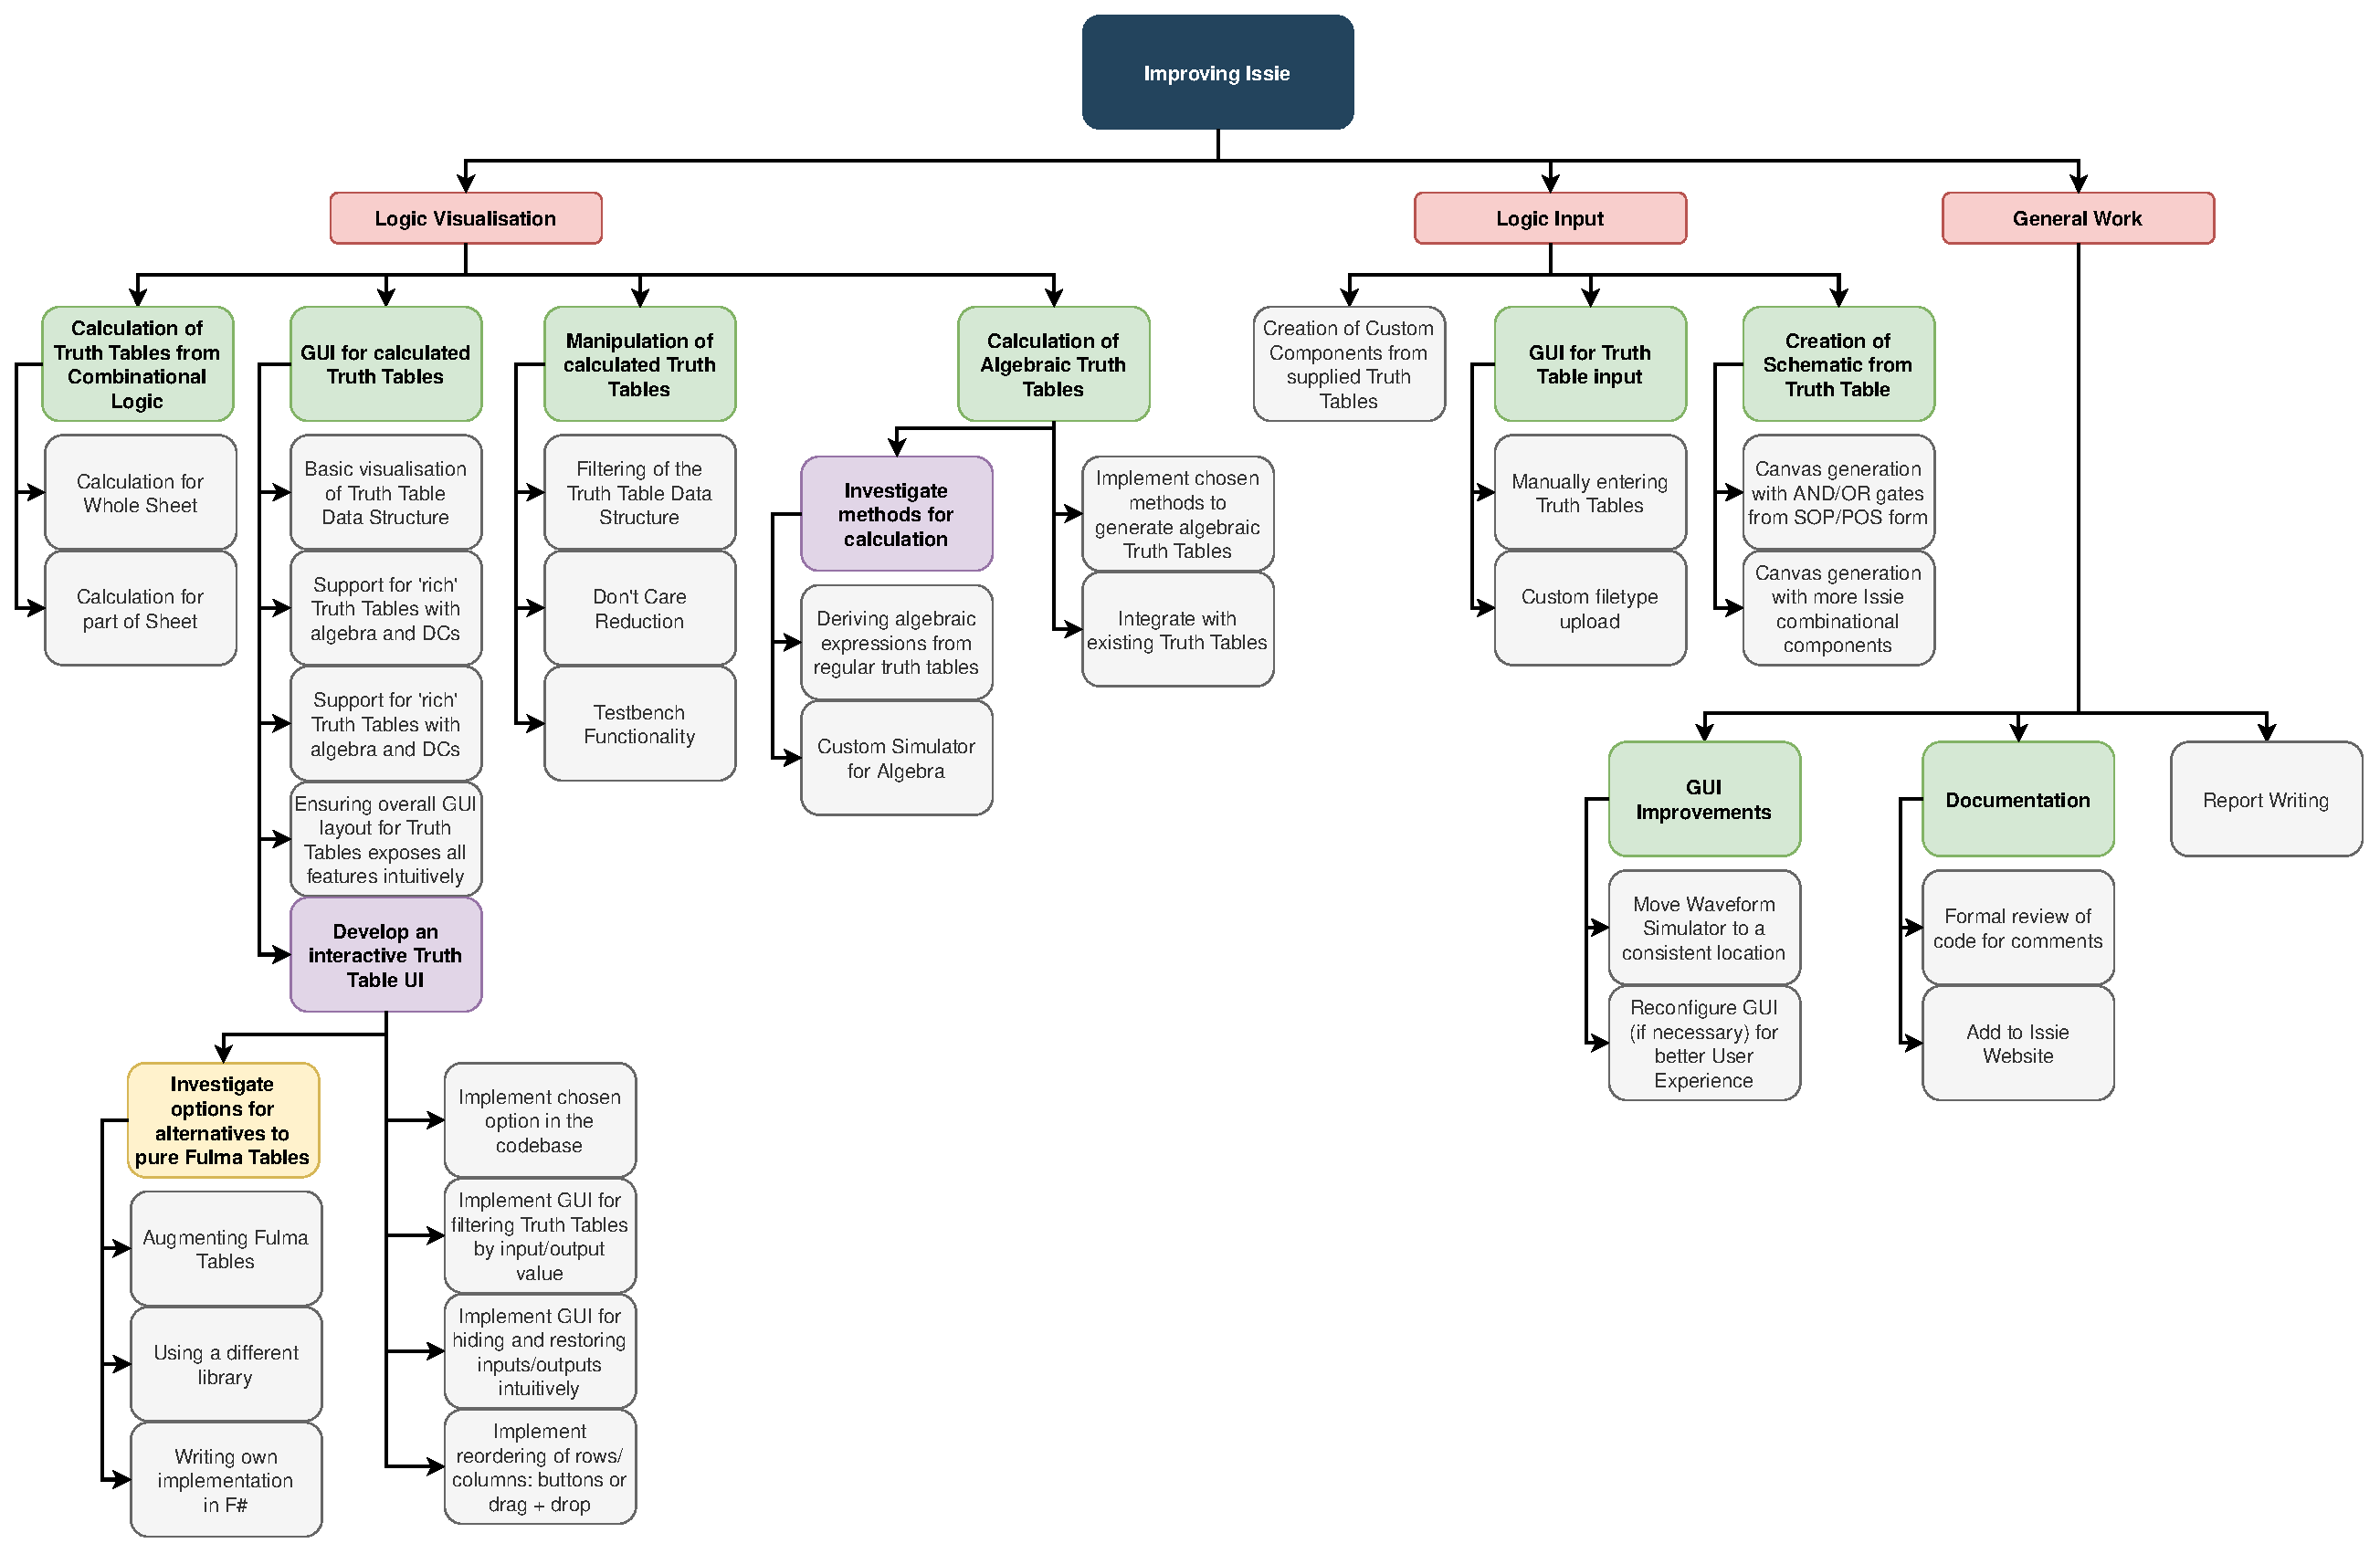
\includegraphics[width=22cm,angle=270,origin=c]{05.ImpPlan/wbs.eps}
%     \caption{Work Breakdown Structure for the Project (Rotated)}
%     \label{fig:wbs}
% \end{figure}

% \begin{figure}
%     \centering
%     \includegraphics*[width=\textwidth]{05.ImpPlan/gantt_update.pdf}
%     \caption{Gantt Chart for the Project}
%     \label{fig:gantt}
% \end{figure}

\section{Filtering with Output Constraints}
While input constraints are applied when generating the input space for performance reasons, output constraints are applied to the generated truth table. This is done for performance reasons; it is quicker to iterate through an existing truth table and filter specific rows compared to re-generating the whole table and only including rows which match the constraints. All output constraints (equality and inequality) are placed in a list, this list is passed to \codestyle{List.fold}, along with the truth table (\codestyle{Map<TruthTableRow,TruthTableRow>}, which is the initial state. Each call of the folder function applies the next output constraint to the Map, which shrinks with every iteration. Figure \ref{fig:outputconsfilter} shows a visual description of this process.

\begin{figure}
    \centering
    \includegraphics[width=0.5\textwidth]{05.ImpPlan/outputconstraints.pdf}
    \caption{Method for Filtering the Truth Table with Output Constraints}
    \label{fig:outputconsfilter}
\end{figure}

\section{Don't Care Reduction}
Truth table reduction using Don't Care terms is implemented using a recursive algorithm which attempts to keep reducing the truth table until there are no redundancies in the table. A recursive function is used as a single row may contain multiple Don't Care terms, meaning that redundancies may still exist in the truth table after a single round of reduction. As discussed in Sections \ref{subsec:dcbackground} and \ref{sec:dcreductionanalysis}, Don't Care reduction in Issie differs from similar logic minimisation techniques as columns in truth tables can have multi-bit values instead of purely zeros and ones.
Issie focuses on teaching digital design principles, therefore on displaying relationships in the logic is more important than achieving the most minimal implementation. All functions related to the reduction of truth tables can be found in the file \codestyle{TruthTableReduce.fs}.
Due to the complex nature of the recursive function, it would be impractical to reduce very large tables. Therefore, only \textbf{non truncated} tables can be reduced using Don't Cares. Larger schematics ought to be reduced algebraically. 

An example of Don't Care Reduction in action is shown in Figure \ref{fig:mux4}. Figure \ref{fig:mux4schematic} shows a schematic in which the Issie component \textit{Mux4} takes 4 2-bit inputs into its data lines, and a 2-bit input into it's select line. The full numeric truth table for this schematic has 1024 rows. Applying the algorithm to the table yields a table (\ref{fig:mux4table}) with only 16 rows: a reduction of over 98\%. Rows in this table have multiple DC terms.

\begin{figure}
     \centering
     \begin{subfigure}[b]{0.45\textwidth}
         \centering
         \includegraphics[width=\textwidth]{05.ImpPlan/mux4.png}
         \caption{Mux4 Schematic}
         \label{fig:mux4schematic}
     \end{subfigure}
     \begin{subfigure}[b]{0.45\textwidth}
         \centering
         \includegraphics[width=\textwidth]{05.ImpPlan/mux4table.png}
         \caption{Reduced Truth Table for the schematic}
         \label{fig:mux4table}
     \end{subfigure}
        \caption{Schematic and Reduced Truth Table}
        \label{fig:mux4}
\end{figure}

\subsection{Prerequisite Concepts}
Prior to explaining the reduction algorithm, certain key concepts regarding truth tables are covered. A DC row is defined as a row that contains Don't Care terms.
\paragraph{Row Equality} 
Truth Table Rows are simply lists of cells, and these lists are compared element-wise to check for row equality. A cell is equal to another cell if they have the same IO and Data values. However, if either of the cells have a Don't Care term, the cells are considered to be equivalent as a Don't Care term can be equal to any value. Two rows can be compared using the \codestyle{rowEquals} function.

\paragraph{Looking up Rows in the Truth Table}
The truth table is implemented as a Map data structure, and therefore has efficient lookups. However, the exisiting \codestyle{Map.tryFind} function uses default F\fsharp equality checking when performing lookups. In order to support DC rows, the equality function \codestyle{rowEquals} should be used. The function \codestyle{tableTryFind} works like \codestyle{Map.tryFind}, but supports querying the table with Don't Care terms in rows. As a Don't Care term represents multiple values, one row can map to multiple rows. Therefore, \codestyle{tableTryFind} returns a list of all output rows that match the input row.

\paragraph{Validity of a Row with Don't Cares}
Within a truth table, a row containing Don't Care terms is considered valid if the relationship it describes is correct -- i.e. is the variable actually redundant in the given input combination. This is tested by finding all output rows that correspond to the input DC row using \codestyle{tableTryFind}. If all of the returned output rows are equal, then the DC row is valid. If not, then it is invalid.

\subsection{Reduction Algorithm}
The algorithm takes an instance of the Truth Table data structure as input, and returns a new instance of the data structure, this time with the \codestyle{DCMap} field populated with a Map. As the algorithm is called recursively on the input data structure, the algorithm first checks if a \codestyle{DCMap} exists. If it does not, then this is the first call and therefore the numeric \codestyle{TableMap} is used. If the field is populated, then this is a subsequent reduction of the \codestyle{DCMap}, so it is used. Following this, the algorithm can be split into three stages:

\subsubsection{Stage 1: Find all valid Don't Care Rows}
\begin{lstlisting}[caption=Finding all DC Rows ,frame=tlrb, language=FSharp, label=lst:alldcrows]{Name}
let allDCRows =
        table.Inputs
        |> List.collect (fun input ->
            inputDCRows input inputConstraints table bitLimit)
\end{lstlisting}
The function \codestyle{inputDCRows} finds all DC rows for a given input. This function is called for each input, and the returned rows are all collected. \codestyle{inputDCRows} first generates all possible DC rows for the input by replacing any numerical values of the given input in the table with a Don't Care term. These possibilities are then validated against the truth table using the function \codestyle{isValidDCRow}, with invalid rows being discarded from the list. This leaves only valid DC rows.

\subsubsection{Stage 2: Find which rows from the Truth Table should remain}
\begin{lstlisting}[caption=Finding which regular rows should remain in the Truth Table ,frame=tlrb, language=FSharp, label=lst:regremain]{Name}
let remainingRegularRows =
        (Map.toList tMap, allDCRows)
        ||> List.fold reduceWithDCRow
\end{lstlisting}
Once all valid DC rows are found, these rows are used to reduce the existing table. The process of reducing the table using DC rows is similar to the process of filtering the table using output constraints. Every row in the truth table is compared to every valid DC row using \codestyle{rowEquals}. If a row in the existing truth table is equal to a DC Row, it means that it is redundant in the table and should be removed. This process returns a list of the rows from the existing truth table that were not made redundant by the DC rows and should therefore remain in the truth table.

\subsubsection{Stage 3: Assembling the Reduced Table and Recursive call}
By combining the DC rows and remaining regular rows, the reduced truth table for this round of reduction can be obtained. However, one round of reduction can only add one Don't Care term to each row. However, certain truth tables may require multiple DC terms in each row to be fully reduced -- Figure\ref{fig:mux4table} is an advantage of this. Therefore, the reduction algorithm is called recursively on the reduced truth table. This chain of recursive calls continues until the reduced tables generated by two successive rounds are found to be equal, as this indicates that the table can be reduced no further. This fully reduced table is returned to the user for viewing.

\section{Algebraic Truth Tables}
Once a truth table has been generated, the user can reduce the number of rows in the table by changing inputs from numerical values to algebraic expressions. Section \ref{sec:algebra_types} discussed in detail the nature of algebraic operators and expressions in Issie, while Table \ref{tab:algebraops} in the Analysis and Design chapter explained what every operator the user may encounter means. Algebraic truth tables are obtained through \textit{Algebraic Simulation}; specific inputs selected by the user are fed to the underlying Fast Simulation as \codestyle{SingleTerm} algebraic expressions, and these expressions propagate through the simulation and are manipulated by operators. The outputs of the simulation are therefore also algebraic expressions, which summarise the output in terms of the input. 

\subsection{Definition of the Algebraic System}
A new system of algebra was created by this project for use in algebraic truth tables in Issie. The aim of the algebra is to clearly communicate the semantic meaning of the combinational logic function described by the schematic. These functions are traditionally defined using Boolean algebra, but this system was deemed unfit for use in algebraic truth tables. Simplified Boolean algebra can describe which operations are being performed on the inputs at a hardware level, but lacks a way to succinctly describe more advanced operations which consist of multiple regular Boolean operations. Arithmetic operations are an example of this. While Issie supports multi-bit inputs and wire buses in logic, traditional Boolean algebra assumes all input variables have a width of 1. Therefore it does not include operators for manipulating buses such as slicing or merging. Due to these reasons, the decision was made to define a new formal language (algebra) which would be a superset of Boolean algebra, adding support for arithmetic and multi-bit bus operations. Formal languages are a set of sequences, or strings over some finite vocabulary \cite{jäger_rogers_2012}, defined using a grammar. The F\fsharp implementation of the algebra differs slightly in some places from the more formal definition described below to allow for easier comprehension and simplification. The F\fsharp type definitions are described in Section \ref{sec:algebra_types}.

\subsubsection{Terminal Symbols}
A terminal symbol is the simplest constituent of an algebraic expression, which cannot be sub-divided or simplified further. In the defined algebra, terminal symbols can be split into two categories. The first category represents the base value type which operations can be performed on. There are two terminal value types in the algebra; these are described in Table \ref{tab:terminals}. The second category consists of the operators which manipulate expressions. These are described in Table \ref{tab:algebraops}.
\begin{table}[!ht]
    \centering
    \scalebox{0.9}{
    \begin{tabular}{|m{2cm}|m{3cm}|m{9cm}|}
    \hline
        \textbf{Symbol} & \textbf{Name in Code} & \textbf{Explanation} \\ \hline
        Variable & \codestyle{SingleTerm} & A symbol representing an algebraic input into the simulation. Any valid IO Label string can be a variable. \\ \hline
        Number & \codestyle{DataLiteral} & A known numerical value in the simulation. Used to represent numerical inputs into the simulation. \\ \hline
    \end{tabular}}
    \caption{Terminal Value Symbols}
    \label{tab:terminals}
\end{table}

\begin{table}[!ht]
    \centering
    \scalebox{0.9}{
    \begin{tabular}{|m{4cm}|m{2.5cm}|m{7.5cm}|}
    \hline
        \textbf{Symbol} & \textbf{Name in Code} & \textbf{Explanation} \\ \hline
        Numeric Addition: $+$ & \codestyle{AddOp} & Binary operator which represents mathematical addition of its two operands. \\ \hline
        Numeric Subtraction: $-$ & \codestyle{SubOp} & Binary operator which represents mathematical subtraction of its right operand from its left operand. \\ \hline
        Bitwise And: $\&$ & \codestyle{BitAndOp} & Binary operator which for a Boolean And between each bit of its operands (bitwise) . \\ \hline
        Bitwise Or: $|$ & \codestyle{BitOrOp} & Binary operator which for a Boolean Or between each bit of its operands (bitwise) \\ \hline
        Bitwise Xor: $\bigoplus$ & \codestyle{BitXorOp} & Binary operator which for a Boolean Xor between each bit of its operands (bitwise) \\ \hline
        Numeric Negation: $-$ & \codestyle{NegOp} & Unary negation operator, indicates that the single operand will have its sign inverted \\ \hline
        Bitwise Not: $\sim$& \codestyle{NotOp} & Unary bitwise Not operator, indicates that all bits of the single operand will be inverted \\ \hline
        Carry Of: $carry()$ & \codestyle{CarryOfOp} & Unary operator which signifies that the result is the single-bit carry-out from an arithmetic expression. This expression is the operand, which is situated in the parentheses. \\ \hline
        Bit Range: $[u:l]$ & \codestyle{BitRangeOp} & Unary operator with two parameters: an upper and lower bound. Indicates that a specified range of bits (inclusive) will be selected from the operand. \\ \hline
        Equals: $==$ & \codestyle{Equals} & Logical operator which checks for equivalence between some algebraic expression and a numeric value. \\ \hline
        Append: $::$ & \codestyle{AppendOp} & Binary operator which joins the bits of the two input operands into one result whose width is the sum of the input widths. The left operand bits become the MSBs, right operand bits become LSBs. \\ \hline
    \end{tabular}}
    \caption{Terminal Operator Symbols}
    \label{tab:algebraops}
\end{table}

\subsubsection{Non-Terminal Symbols}
Non-terminal symbols are constructs that appear within algebraic expressions which can eventually be simplified/replaced with terminal symbols.

\begin{table}[!ht]
    \centering
    \scalebox{0.9}{
    \begin{tabular}{|m{4cm}|m{3cm}|m{7cm}|}
    \hline
        \textbf{Symbol} & \textbf{Name In Code} & \textbf{Explanation} \\ \hline
        Binary Operator & \codestyle{BinaryOp} & Defines all binary operators (operators which take two operands) and can be substituted by any. \\ \hline
        Unary Operator & \codestyle{UnaryOp} & Defines all unary operators (operators which take one operand) and can be substituted by any. \\ \hline
        Binary Expression & \codestyle{BinaryExp} & Defines an expression in which a binary operator acts on its operands. \\ \hline
        Unary Expression & \codestyle{UnaryExp} & Defines an expression in which a unary operator acts on its operands. \\ \hline
        Comparison Expression & \codestyle{ComparisonExp} & Defines an expression in which a comparison operator compares a symbol with a value \\ \hline
        Expression & \codestyle{FastAlgExp} & Highest level non-terminal symbol, defines all expressions in the simulation. \\ \hline
    \end{tabular}}
    \caption{Non-Terminal Symbols}
    \label{tab:nonterminals}
\end{table}

\subsubsection{Production Rules and Start Symbol}
Production rules in grammars have the form $\alpha \rightarrow \beta$, understood as $\alpha$ may be replaced by $\beta$, where $\alpha$ and $\beta$ are sequences comprising symbols from the terminal and non-terminal set of symbols \cite{jäger_rogers_2012}. These production rules can be described in \textit{Backus-Naur Form} (BNF); this is a format for presenting grammars often used when defining programming languages. In BNF, non-terminal symbols, which are called \textit{metalinguistic variables} are enclosed in brackets to differentiate them from terminal symbols. The symbol $::=$ indicates \textit{metalingustic equivalence}: whatever is to the left of the symbol can be substituted by whatever is to the right. The symbol $|$ implies a choice of equivalences (akin to a logical OR) -- i.e. something can be substituted by option 1 or option 2. Finally, concatenation of symbols (linking) is achieved by placing them next to one another \cite{bnf}. The production rules for the algebra, defined in BNF are: 

%\textit{Note: the symbol} \textbf{|} \textit{is used for bitwise Or, but is also used in BNF. Therefore, the bitwise Or symbol will be enclosed in quotes when used in the definition} \textbf{"|"}. 
\setlength{\grammarparsep}{0.25cm}   % vertical distance between production rules
\setlength{\grammarindent}{4.5cm}
\begin{center}
\begin{grammar}
    <binary operator> ::= "+" \alt "-" \alt "\&" \alt "|" \alt "\bigoplus"

    <unary operator> ::= "-" \alt "\sim" \alt "carry()" \alt "[u:l]"

    <comparison operator> ::= "=="
    
    <binary expression> ::= <expression> <binary operator> <expression>
    
    <unary expression> ::= <unary operator> <expression>
    
    <comparison expression> ::= <expression> <comparison operator> "number"
    
    <expression> ::= "variable" \alt "number" \alt <binary expression> \alt <unary expression> \alt <comparison expression>
\end{grammar}
\end{center}
Grammars will generally build up into a tree-like structure, with the terminal symbols as its leaves and non-terminals as intermediate nodes in the tree. The root of this tree is known as the \textbf{start symbol}. In a formal grammar, it should be possible to arrive a sequence of terminal symbols by repeatedly and/or recursively applying the defined production rules to the start symbol. In the case of the defined algebra, the start symbol is the \textit{expression}.
% \begin{bnf*}
%     \bnfprod{binary operator}
%         {\bnfts{+} \bnfor \bnfts{-} \bnfor \bnfts{\&} \bnfor \bnfts{"|"} \bnfor \bigoplus}\\
%     \bnfprod{unary operator}
%         {\bnfts{-} \bnfor \sim \bnfor \bnfts{carry()} \bnfor \bnfts{[u:l]}}\\
%     \bnfprod{comparison operator}
%         {==} \\
%     \bnfprod{binary expression} {\bnfpn{expression} \bnfsp \bnfpn{binary operator} \bnfsp \bnfpn{expression}}
%     \bnfprod{unary expression} {\bnfpn{unary operator} \bnfsp \bnfpn{expression}} \\
%     \bnfprod{comparison expression} {\bnfpn{expression} \bnfsp \bnfpn{comparison operator} \bnfsp \bnfts{number}} \\
%     \bnfprod{expression}
%         {\bnfts{variable} \bnfor \bnfts{number} \bnfor \bnfpn{binary expression}}
%         \bnfmore{\bnfor \bnfpn{unary expression} \bnfor \bnfpn{comparison expression}}
        
% \end{bnf*}
\subsection{Implementing Algebra}

In order to enable algebraic simulation, the Fast Simulation code was extended by the project to support algebraic inputs and reduction. 
Prior to the addition of algebra, the primary data type used to represent values in the Fast Simulation was \codestyle{FastData}, a record type containing a value and its width. \codestyle{FastData} was wrapped in the type \codestyle{FData}; the code in the Fast Simulation used the \codestyle{FData} type in the implementation. This was done to make the logic easier to extend, as if the logic ever had to handle two types of data \codestyle{FData} could simply be transformed in to a Discriminated Union of the usable types. This is an example of \textit{Extensibility}, one of Issie's core principles, in action. The approach of turning \codestyle{FData} into a DU type was adopted by the project -- the change in the type definition can be seen in Listing \ref{lst:fdata}. \codestyle{FData}, the data type used in all simulation logic, can either be numeric data (as it was before), or an algebraic expression. Following this change in definition, an extensive refactoring process had to take place to fix over 100 compiler errors caused by functions expecting to be given data resembling \codestyle{FastData} as input, but actually given a discriminated union. Only after this exercise was completed, could the true implementation of algebraic simulation begin. 
\begin{lstlisting}[caption=Change in definition of \codestyle{FData},frame=tlrb, language=FSharp, label=lst:fdata]{Name}
// Old Definition
type FData = FastData

// New Definition
type FData = | Data of FastData | Alg of FastAlgExp
\end{lstlisting}

When the Fast Simulation is built, all components in the schematic are placed in a specific order which allows them to be reduced. This reduction process involves propagating values from the input ports of a component to its output ports, which are propagated to the input ports of the next component in line. This is repeated until the end of the list is reached.
The function responsible for propagating these values is \codestyle{fastReduce}. It consists of a large Pattern Match expression, with defined behaviour for how each component transforms its input values into output values. Previously, the values at the input ports could only be \codestyle{FastData}, however after the change in definition they could also be algebraic expressions. Therefore, the defined behaviour for every component specified in \codestyle{fastReduce} had to be extended to support algebraic expressions. Table \ref{tab:fastReduce} summarises the extensions to \codestyle{fastReduce} which enabled algebraic simulation. Some components have multiple cases (a '-' signifies the default case) -- this is because certain algebraic relationships can be inferred during the reduction algorithm and the correct result is therefore propagated. An example of this is when one of the inputs to an \textit{NbitsAdder} component is a expression with a not operator, and the carry-in is 1. The Not operator symbolises a bit-inversion, so adding 1 to that results in a 2's complement representation of the expression the Not operator was applied to. This means that the adder is now performing subtraction: $A + \Bar{B} + 1 = A - B$. The advantage of this approach is that it is extensible; the algebraic simulation can be made smarter by simply programming in more specific cases. There are specific cases where algebraic simulation has not been implemented, such as for sequential components or for when algebra is passed to the select port of a multiplexer. In these cases, an \codestyle{AlgebraNotImplemented} exception, which contains a \codestyle{SimulationError} is raised. This error is then returned to the user.

% \begin{table}[!ht]
%     \centering
%     \scalebox{1}{
%     \begin{tabular}{|m{2cm}|m{4cm}|m{8cm}|}
%     \hline
%         \textbf{Component} & \textbf{Case} & \textbf{Defined Behaviour} \\ \hline
%         Not & - & Apply the unary Not operator to the algebraic expression. \\ \hline
%         BusSelection & - & Apply the unary BitRange operator to the expression based on width and LSB supplied. \\ \hline
%         BusCompare & - & Apply the comparison operator to the expression, comparing it to the supplied value. \\ \hline
%         \shortstack{And, Or,\\ Xor} & - & Apply the relavent binary operator to both expressions \\ \hline
%         \shortstack{Nand, Nor,\\ Xnor} & - & Apply the the binary operator for the uninverted versions of the gates, and then apply the unary Not operator to the result. \\ \hline
%         \multirow{2}{*}{\shortstack{Mux2, Mux4\\ Mux8}} & Data inputs are algebra or numeric, Select input is numeric & If the select input is 0, propagate the expression/number connected to port 0. If select input is 1, propogate the expression/number connected to port 1 and so on… \\ \cline{2-3}
%         ~ & Select input is algebra & Algebra not allowed at select port of multiplexer. Raise AlgebraNotImplemented exception. \\ \hline
%         \multirow{2}{*}{\shortstack{Demux2,\\ Demux4,\\ Demux8}} & Data input is algebra or numeric, Select input is numeric & Propagate the expression/value to the correct output corresponding to the Select value. \\ \cline{2-3}
%         ~ & Select input is algebra & Algebra not allowed at select port of demultplexer. Raise AlgebraNotImplemented exception. \\ \hline
%         \multirow{3}{*}{NbitsAdder} &  The carry-in is 1, and one of the inputs is an expression with a Not operator & This is subtraction, apply the binary Subtraction operator to the two inputs. \\ \cline{2-3}
%         ~ & Out of the three inputs, two are numeric, one is algebraic & Add the two numeric values together, and then apply the binary Add operator to the expression and the sum. \\ \cline{2-3}
%         ~ & - & Apply the binary Add operator to two inputs, and then apply a second Add operator to the first expression and the third input. \\ \hline
%         \multirow{2}{*}{NbitsXor} & One input is algebra, the other is -1. & This is bit inversion, apply the unary Not operator to the input. \\ \cline{2-3}
%         ~ & - & Apply the binary Xor operator to the inputs. \\ \hline
%         \multirow{3}{*}{SplitWire} & Input is an algebraic expression with a BitRange operator & Change the values in the bit range operator according to which bits are going to output ports 0 and 1. \\ \cline{2-3}
%         ~ & Input is an algebraic expression with a Not opeartor & Apply the BitRange operator to the expression inside the Not operator, as bit ranges bind closer. \\ \cline{2-3}
%         ~ & - & Apply the unary BitRange operator to the expression, with different ranges for output ports 0 and 1. \\ \hline
%         \multirow{3}{*}{MergeWires} & Both inputs are append expressions (a list of appened expressions) & Join the two lists in the correct order, and then check if any BitRanges can be joined. \\ \cline{2-3}
%         ~ & One of the inputs is an append expression & Add the new element to the head or tail of the list depending on the order, and then check if any BitRanges can be merged. \\ \cline{2-3}
%         ~ & - & Put the two inputs in a list together in the correct order, and check if any BitRanges can be merged. \\ \hline
%         \shortstack{Any other\\ components} & - & These are sequential components which should not accept algebra, raise an AlgebraNotImplemented exception. \\ \hline
%     \end{tabular}}
%     \caption{New additions to the defined behaviour for each components in \codestyle{fastReduce}}
%     \label{tab:fastReduce}
% \end{table}

% Alongside interpretation of cases during algebraic reduction, informative algebraic relationships are also calculated once the simulation is completed by evaluating the expressions using the \codestyle{evalExp} function. This function recursively evaluates the sub-expressions which make up the often large and complex output expression. The cases that are caught and evaluated by this function are:
% \begin{enumerate}
%     \item Double inversion (a not operator acting on a not operator) is replaced with the underlying expression
%     \item Double negation (a negation operator acting on a negation operator) is replaced with the underlying expression
%     \item And operation between an expression and 0 evaluates to 0, while And with 1 always evaluates to the expression
%     \item Or operation between an expression and 0 evaluates to the expression, while Or with 0 always evaluates to 1
%     \item Xor operation between an expression and 0 evaluates to the expression, while Xor with 1 evaluates to the inverse of the expression (Not operator on expression)
%     \item Bitwise logical operations are detected -- if a logical operation such as an And is performed on every bit of two multi-bit inputs, this pattern will be recognised as an And between the two inputs.
% \end{enumerate}
% Similar recursive functions are also used to calculate the width of a given expression, as well as convert an expression to a string for display purposes.

\section{Sorting Truth Tables}
In Issie, the order in which rows appear in the truth table can be set by the user by clicking the up/down arrows in the heading of each column of the table. The initial order of the rows in the truth table is seemingly arbitrary; this is because truth tables are generated as F\fsharp Maps, and the order of the keys in the Map is determined by F\fsharp's generic comparison \cite{fsmaps}. As Maps cannot retain a custom set order, a different collection type had to used for sorting the truth table. Therefore, the Map is converted row-wise into a list of \codestyle{TruthTableRow}s, where each individual \codestyle{TruthTableRow} is formed by appending each input row to its corresponding output row. This list representation is the last stage in the truth table caching strategy, which will be discussed further in Section \ref{sec:cachingTT}.

When the user clicks a specific arrow in the truth table to sort it, two messages are sent to the Update function. The first message, \codestyle{SetTTSortType}, contains two pieces of information: which IO should the table be sorted by, and whether this is in ascending or descending order. This information is updated in the Model (under field \codestyle{TTSortType}) . The second message marks the truth table as being out of date, with the reason that it must be sorted. The reason for why the setting of the sort type is separated from actual sorting of the truth table is explained in detail in \ref{sec:cachingTT}. The actual sorting process begins by looking up the current Sort Type in the model -- if there is some then the truth table is sorted according to it. 
F\fsharp provides library functions for sorting lists in $O(n log(n))$ time using QuickSort; one such function is \codestyle{List.sortWith}, which allows the developer to define a custom comparison function for two elements in the list. A custom comparison function for comparing two \codestyle{TruthTableRow}s is required, as the generic comparison offered by F\fsharp does not compare rows correctly. When the truth table is being sorted by some IO $X$, the position of a given row in the sorted truth table is dependent on the value of $X$ in that row. Therefore, it was determined that the process of comparing two rows involved first extracting the appropriate \codestyle{CellData} values for the IO, and comparing those.

\subsection{Comparison Function for \codestyle{CellData}}
The following comparison rules were determined for data in truth table cells:
\begin{enumerate}
    \item Don't Care (DC) Terms are larger than Algebraic Expressions, which are larger than numeric values.
    \item Algebraic terms are compared based on their alphabetical order, so "A" < "B".
    \item Numerical terms are compared based on their values, as expected for numbers: 0 < 1 < 2 etc.
\end{enumerate}

Functions for comparing two values in F\fsharp have the following signature:
\begin{center}
    \codestyle{'T -> 'T -> int}
\end{center}
This means that the comparison function takes the two objects to compare as arguments, and returns an integer which signifies which argument was larger than the other. A positive return values indicates that the first argument is greater than the second, a negative return value suggests that the second argument is greater than the fist, and a return value of 0 indicates that the values are equal. The three comparison rules were implemented as a comparison function with the aforementioned signature; this can be seen in Listing \ref{lst:compareCellData}. The alphabetical and numerical comparisons are handled with F\fsharp's built-in \codestyle{compare} function.

\begin{lstlisting}[caption=Function to compare two \codestyle{CellData} values,frame=tlrb, language=FSharp, label=lst:compareCellData]{Name}
let compareCellData (cd1: CellData) (cd2: CellData) =
    match cd1, cd2 with
    | DC, DC -> 0
    | DC, _ -> 1
    | _, DC -> -1
    | Algebra _, Bits _ -> 1 
    | Bits _, Algebra _ -> -1
    | Algebra a1, Algebra a2 -> 
        compare a1 a2
    | Bits wd1, Bits wd2 ->
        (convertWireDataToInt wd1, convertWireDataToInt wd2)
        ||> compare
\end{lstlisting}

\section{Truth Table Caching and Order of Operations} \label{sec:cachingTT}
So far, five user operations that change the truth table data structure have been discussed. These are summarised in Table \ref{tab:ttOps}. From inspecting this table, it can be seen that only changing the input constraints or changing algebraic inputs requires the truth table to be re-generated. The rest of the operations simply transform the existing truth table. For this reason, the whole process of serving the user a truth table is split into various parts, each of which execute in a specific order, only do as much work as necessary, and cache their results. This whole process is described in Figure \ref{fig:ttOps}. There is a strict order of operations; first the truth table is regenerated, then it is filtered, and then it is sorted. Column hiding occurs after sorting, but this does not change the truth table data structure itself, and is therefore discussed in Section \ref{subsec:colhide}. If the truth table is to be reduced with Don't Cares, then the filtering stage filters the \codestyle{DCMap} instead of the \codestyle{TableMap}, and this propagates through the subsequent stages. The result of each operation is stored in the \codestyle{TruthTable} data structure, which is itself stored in the model. Once a given operation has completed and stored its result, it calls the next step using a \textit{Command}. In the MVU architecture, Commands are used to send a message to the next call of the update function. In the context of the system in Figure \ref{fig:ttOps}, using commands means that the next operation in the order is executed during the next call of the Update function. This ensures that the next operation uses the newly stored result from the current operation. 

\begin{table}[!ht]
    \centering
    \begin{tabular}{|p{4cm}|p{9cm}|}
    \hline
        \textbf{Operation} & \textbf{Summary} \\ \hline
        Changing Input Constraints & The truth table is re-generated, taking the new input constraints into account. \\ \hline
        Changing Output Constraints & The existing truth table is filtered, with only rows which fulfil the constraints allowed to remain. \\ \hline
        Changing Algebraic Inputs & The truth table is re-generated, taking the new algebraic and numeric inputs into account. \\ \hline
        Don't Care Reduction & The existing truth table is reduced down into an alternate form with redundancies removed and replaced with DC Terms. \\ \hline
        Sorting & The existing truth table rows are reordered to reflect the user's chosen sorting method. \\ \hline
    \end{tabular}
    \caption{Summary of operations which change the \codestyle{TruthTable} data structure}
    \label{tab:ttOps}
\end{table}

The reason for this system, as opposed to one where all of the operations are performed in one go, is best explained through an example.
Suppose the truth table has two output constraints $X=0$ and $Y = 0$ applied to it, and the user subsequently deletes the latter. Rather than re-generate the truth table from scratch and then apply the new set of output constraints, Issie simply uses the cached version of the full table (stored in \codestyle{TableMap}), and applies the new output constraint set to that. This approach reduces the time-penalty for the given operation, as unnecessary steps are cut out.

Another key feature of the system is that the parameters for each operation are stored independently in the model. When an operation parameter, such as the algebraic input set or the constraint set changes, the update function first updates the stored parameter value in the model, then sends a command carrying the message to execute the appropriate operation.
Storing the parameters has two uses; the first is that it allows for them to be displayed and tracked. For example, constraints that are currently being applied are displayed to the user using tags, and are used to validate new ones. However, the more interesting effect of this concept is that users do not lose their preferences no matter what other operations they do on the truth table. This too is best explained through an example. Suppose the truth table from before still has the output constraint $X=0$ applied to it, but the user then chooses to add a new input constraint $A=0$. When the user clicks the \textit{Add} button in the popup, the \codestyle{AddInputConstraint} message, which contains the new constraint, is sent -- this is then processed by the Update function which stores it in the Model. Following this, a command containing the message \codestyle{RegenerateTruthTable} is sent.  In the next call of the Update function, the truth table is regenerated, and once this is completed the rest of the stages execute in the correct order. As the output constraints are stored independently in the model, the system remembers to apply $X=0$ to the new \codestyle{TableMap}. In this vein, any pre-existing sorting method, column order, or hidden columns are also preserved after the re-generation. This means that \textbf{only} the operation instructed by the user occurs, meaning that the user is not left confused by unintended side effects of their interactions with the truth table.


\begin{figure}[h]
    \centering
    \includegraphics[width=\textwidth]{05.ImpPlan/tableoperations.pdf}
    \caption{How operations update the Truth Table}
    \label{fig:ttOps}
\end{figure}

\section{Rendering the Truth Table}
Displaying a truth table involves taking the \codestyle{TruthTable} data structure and transforming it into a \codestyle{ReactElement} which can be rendered by React. Two methods were considered for this task; Fulma tables and CSS Grids. The former was used initially, but due to limitations that will be explained in this section, the latter was eventually favoured.

\subsection{Method 1: Using Fulma Tables}
Fulma, as described in \ref{subsec:fulma}, is an F\fsharp library which provides ready-to-use front-end components for Fable React applications. Component libraries like Fulma have many advantages over plain HTML components that are manually styled using CSS. All Fulma components are pre-styled with specific themes, therefore consistently using Fulma components across an application provides consistency in styling. Additionally, components have style modifiers which can be easily selected by the developer without manually implementing them in CSS. For example, a Fulma table can be made zebra-striped using the \codestyle{Table.IsStriped} modifier \cite{fulmatable}. Certain behaviour, such as automatic re-sizing and automatic wrapping of content is also implemented in Fulma tables. Due to these advantages, and given that Fulma components are used extensively throughout Issie, Fulma tables were initially chosen for rendering the truth table.
Listing \ref{lst:fulmatable} in Section \ref{subsec:fulma} shows the syntax for generating a table with Fulma. A table heading tag (\codestyle{thead}) contains a table row tag (\codestyle{tr}), which contains the numerous heading cells (\codestyle{th}) in the column-order they will be displayed. Similarly, a table body \codestyle{tbody} tag wraps multiple table row tags, which wrap multiple table data \codestyle{td} tags. This tag hierarchy is akin to a nested list representation of a table; therefore it was easy to convert a list representation of the truth table into a Fulma table. Each \codestyle{TruthTableCell} was be mapped to a \codestyle{td} component, and the row containing those cells as mapped to a \codestyle{tr} component.

\subsubsection{Issue with using Fulma Tables}
Table components (both Fulma and HTML) have one major limitation: they are not interactive. The positioning of content in the table is solely dependent on the order during the definition of the table. Once the table is defined, there is no way to change the order in which rows or columns appear in the table at render time. Therefore, all user operations on the table must update the underlying truth table data structure. The previous Section (\ref{sec:cachingTT}) showed how truth tables operations are executed and cached in the delivered version of Issie;  however when tables were rendered using Fulma, hiding/un-hiding columns and changing the order of columns used to also change the \codestyle{TruthTable} data structure and cache the result. For example, when a user moved a column, the order of cells in every \codestyle{TruthTableRow} was changed to reflect the new order. This process involved first copying the sorted list representation into an array, then mutating the array to match the IO order defined by the user. The effect of the quadratic time complexity, coupled with the repeated copying of data and slow element-wise access of lists, was that re-ordering operations on large truth tables (1024 rows, more than 5 columns) took an average of 608.4ms. According to Robert Miller \cite{Miller1968ResponseTI}, such a delay does not appear instantaneous to the user and can therefore make the application feel sluggish rather than responsive. The performance of this method was deemed unacceptable, as requirement \textbf{E1.8} clearly states that graphical manipulation operations must appear instantaneous. Therefore, an alternative approach was considered.

\begin{table}[!ht]
    \centering
    \begin{tabular}{|l|l|l|l|l|l|l|}
    \hline
        Method & Trial 1 & Trial 2 & Trial 3 & Trial 4 & Trial 5 & Average \\ \hline
        Method 1 & 607 & 605 & 611 & 610 & 609 & 608.4 \\ \hline
        Method 2 & 21 & 25 & 22 & 23 & 27 & 23.6 \\ \hline
    \end{tabular}
    \caption{Time taken to move a column in a Truth Table under different methods (ms)}
    \label{tab:colOps}
\end{table}

\subsection{Method 2: Using CSS Grids}
The CSS Grid layout \cite{cssgrids} is a system which allows the developer to define the positioning of specific elements in two-dimensions. Unlike tables, where the positioning of elements is defined inline in the HTML using tags, all display properties of grid elements such as positioning, size, and behaviour are defined within a CSS style. Each grid element is therefore defined within a \codestyle{div} with the appropriate style applied to it. The advantage of this is that changing element positioning does not require changing the underlying data structure and rebuilding the grid -- simply updating the styles will change how the grid is rendered. This ultimately means that grids can be made interactive while tables can not. CSS grids were chosen due to this interactivity property, as it would greatly speed up column hiding and re-ordering as manipulation of the truth table data structure would no longer be required. This hypothesis was proven to be true; Table \ref{tab:colOps} compares the time taken to column move a column under both methods, and shows that manipulating CSS styles is significantly faster than changing the underlying data structure. One of the reasons why Fulma tables were initially chosen was that they would maintain UI consistency with the numerous other Fulma components used in the application. To keep up this UI consistency, the implemented grid has been styled to mimic the look and feel of Fulma tables. 

When the truth table is initially generated, all the IOs in the truth table are arranged in the default simulation order. All of the IOs in the truth table are extracted in this initial order using the \codestyle{TruthTable.IOOrder} member function. Listing \ref{lst:colStyles} shows how a mapping between each of these IOs and a list of CSS Properties is created. The \codestyle{ttGridColumnProps} returns the appropriate CSS Properties for each IO; most of these properties relate to formatting and appearance, however the \codestyle{GridColumnStart} and \codestyle{GridColumnEnd} properties are dependent on the index of the IO. These properties determine the position of an element in the truth table. The reason for why the Start position has 1 added to it is that CSS Grids begin indexing from 1, while F\fsharp lists begin indexing from 0. This Map is then stored in the Model as \codestyle{TTGridStyles} for use during the truth table viewing process, which turns the truth table data structure into a React Element. The last two properties: \codestyle{OverflowX} and \codestyle{OverflowWrap} are responsible for ensuring that long algebraic expressions wrap to the next line in the truth table instead of overflowing the cell that contains them.
\begin{lstlisting}[caption=Generating CSS Properties for each IO,frame=tlrb, language=FSharp, label=lst:colStyles]{Name}
let ttGridColumnProps index = [
    Border "1px solid gray"
    Padding "7px"
    FontSize "18px"
    TextAlign TextAlignOptions.Left
    GridColumnStart <| string (index+1)
    GridColumnEnd <| string (index+2)
    OverflowX OverflowOptions.Auto
    OverflowWrap "break-word"
]

let colStyles = 
    tt.IOOrder
    |> List.mapi (fun i io -> (io,ttGridColumnProps i))
    |> Map.ofList 
\end{lstlisting}

When the truth table is viewed, each \codestyle{TruthTableCell} is transformed into a \codestyle{div} instead of a \codestyle{td}. The style applied to the \codestyle{div} is obtained by looking up the \codestyle{CellIO} in the \codestyle{TTGridStyles} Map which was calculated and stored during initial generation. All of these individual grid elements are wrapped in a container \codestyle{div}, which is styled property \codestyle{Display DisplayOptions.Grid} to indicate that it is the element that contains the grid. Any subsequent manipulations to the position or visibility of specific IOs in the table can be achieved by updating the \codestyle{TTGridStyles} Map rather than the truth table itself. The displayed truth table itself is zebra-striped; the background colour of rows alternates between white and off-white. This is done to improve the clarity and readability of the truth table. A study of 244 people concluded that task performance when using zebra-striped tables is better, or at least no worse than alternative table styles \cite{zebrastripes}.

\section{Column-based Operations}
Operations on the truth table in Issie can be divided into three classes: regenerative, row-based and column-based. Row-based operations manipulate the truth table data structure because they filter or re-order rows based on the specific values stored in cells in each row. As truth tables are stored row-wise in both Map and List representations, manipulating rows is relatively inexpensive. Column-based operations on the other hand do not require reading values from the truth table itself, and are more expensive than row-based operations. For this reason, they are carried out by manipulating the CSS applied to grid elements. As discussed in the previous section, the styles for each column in the truth table are stored in the \codestyle{TTGridStyles} Map, which maps an IO to a list of CSS properties. Different column-based operations update the stored property list in the map accordingly. 

\subsection{Moving Columns}
Truth table columns can be moved using the left and right arrows on either side of the IO Label in the heading of each column. The current order of the columns is stored in the model under the field \codestyle{TTIOOrder}; this is an array of IOs in the order they currently appear in the truth table. When the user clicks an arrow to move a column, the message \codestyle{MoveColumn}, containing the IO and the direction it moves (right or left), is sent. When this message is processed, \codestyle{TTIOOrder} is mutated to reflect the new order. The styles map \codestyle{TTGridStyles} is also updated to reflect the new position of the column in question. During the next view function call, the updated styles will be applied to the grid elements, resulting in the order changing on the user's screen at render-time.

\subsection{Hiding Columns} \label{subsec:colhide}
Using the toggles in the \textit{Hide/Un-hide Columns} menu section, users can change the visibility of output columns in the truth table. The list of IOs whose columns are hidden is stored in the model under the field \codestyle{TTHiddenColumns}. Toggling column visibility to \textit{Hidden} adds the respective IO to the list, and toggling it back to \textit{Visible} removes it from the list. Once this field is updated, a command containing the message \codestyle{HideTTColumns} is issued, meaning that the styles are updated in the next call of the update function. The style corresponding to a hidden IO is updated with the CSS properties shown in Listing \ref{lst:hiddenStyles}. Each hidden column is moved to the end of the grid (hence the requirement for the \codestyle{gridWidth} argument), given a width of 0, and has its \codestyle{visibility} property set to hidden, obscuring it from view. The styles of the remaining visible columns are also updated so that there are no visible gaps in the truth table. A key detail of this system is that the IO itself is not removed from the stored \codestyle{TTIOOrder} -- only its style is changed. This means that when the IO is eventually un-hidden, it will re-appear in the same place as it was before, maintaining continuity.

\begin{lstlisting}[caption=Generating CSS Properties for a Hidden IO,frame=tlrb, language=FSharp, label=lst:hiddenStyles]{Name}
let ttGridHiddenColumnProps gridWidth= [
    GridColumnStart (string <| gridWidth + 1)
    GridColumnEnd (string <| gridWidth + 2)
    Width 0
    OverflowX OverflowOptions.Hidden
    Visibility "hidden"
]
\end{lstlisting}